\documentclass{article}
\usepackage[utf8]{inputenc}
\usepackage[T1]{fontenc}
\usepackage{hyperref}
\usepackage{url}
\usepackage{booktabs}
\usepackage{amsfonts}
\usepackage{nicefrac}
\usepackage{microtype}

\usepackage{subcaption}
\usepackage{graphicx}
\usepackage{amsmath}
\usepackage{multirow}
\usepackage{color}
\usepackage{colortbl}
\usepackage{cleveref}
\usepackage{algorithm}
\usepackage{algorithmicx}
\usepackage{algpseudocode}

\DeclareMathOperator*{\argmin}{arg\,min}
\DeclareMathOperator*{\argmax}{arg\,max}

\graphicspath{{}}

\begin{filecontents}{references.bib}
@article{goessling2024record,
  author = {Goessling, Helge F. and Reick, Christian H.},
  title = {The record-breaking North Atlantic sea-surface temperature anomaly of 2023},
  journal = {Journal of Climate},
  year = {2024},
}

@article{goessling2024unexplained,
  author = {Goessling, Helge F. and Kadow, Christopher and Reick, Christian H.},
  title = {The unexplained persistence of the 2023 North Atlantic warm anomaly},
  journal = {Geophysical Research Letters},
  year = {2024},
}

@article{goren2014satellite,
  author = {Goren, Tom and Rosenfeld, Daniel},
  title = {Satellite observations of cloud regime transitions and aerosol-cloud interactions},
  journal = {Atmospheric Chemistry and Physics},
  year = {2015},
  volume = {15},
  pages = {4357--4373},
}

@article{gryspeerdt2021,
  author = {Gryspeerdt, Edward and Goren, Tom and Sourdeval, Olivier and Quaas, Johannes and Mülmenstädt, Johannes and Dipu, Sudhakar and Unglaub, Claudia and Gettelman, Andrew},
  title = {Constraining the aerosol influence on cloud fraction with satellite observations},
  journal = {Atmospheric Chemistry and Physics},
  year = {2021},
  volume = {21},
  pages = {3871--3891},
}

@article{hannart2016causal,
  author = {Hannart, Alexis and Pearl, Judea and Otto, Friederike E. L. and Naveau, Philippe and Ghil, Michael},
  title = {Causal counterfactual theory for the attribution of weather and climate-related events},
  journal = {Bulletin of the American Meteorological Society},
  year = {2016},
  volume = {97},
  pages = {99--110},
}

@article{hershbach2020era5,
  author = {Hersbach, Hans and Bell, Bill and Berrisford, Paul and Hirahara, Shoji and Horányi, András and Muñoz-Sabater, Joaquín and Nicolas, Julien and Peubey, Carole and Radu, Raluca and Schepers, Dinand and others},
  title = {The ERA5 global reanalysis},
  journal = {Quarterly Journal of the Royal Meteorological Society},
  year = {2020},
  volume = {146},
  number = {730},
  pages = {1999-2049}
}

@article{higgins2017beta,
  author = {Higgins, Steven I. and O'Hara, Robert B. and Römermann, Christine},
  title = {Beta-diversity of plant communities in relation to climate change},
  journal = {Global Change Biology},
  year = {2017},
  volume = {23},
  number = {8},
  pages = {3210-3221}
}

@article{ipcc2021ar6,
  author = {{IPCC}},
  title = {Climate Change 2021: The Physical Science Basis. Contribution of Working Group I to the Sixth Assessment Report of the Intergovernmental Panel on Climate Change},
  journal = {Cambridge University Press},
  year = {2021},
  pages = {1-3949}
}

@article{jakob2003objective,
  author = {Jakob, Christian and Small, Justin D. and Tselioudis, George},
  title = {An objective classification of Southern Ocean cloud regimes},
  journal = {Journal of Climate},
  year = {2020},
  volume = {33},
  number = {12},
  pages = {5181-5196}
}

@article{jakob2012regime,
  author = {Jakob, Christian and Tselioudis, George and Rossow, William B.},
  title = {Cloud-regime-dependent climate feedbacks in a warming climate},
  journal = {Nature Climate Change},
  year = {2018},
  volume = {8},
  pages = {234-239}
}

@article{kay2015community,
  author = {Kay, J. E. and Deser, C. and Phillips, A. and Mai, A. and Hannay, C. and Strand, G. and Arblaster, J. M. and Bates, S. C. and Danabasoglu, G. and Edwards, J. and Holland, M. and Kushner, P. and Lamarque, J.-F. and

@article{loeb2021ceres,
  author = {Loeb, Norman G. and Johnson, Gregory C. and Thorsen, Tyler J. and Lyman, John M. and Rose, Fred G. and Kato, Seiji and Doelling, David R.},
  title = {Satellite and Ocean Data Reveal Marked Increase in Earth's Heating Rate},
  journal = {Geophysical Research Letters},
  year = {2021},
  volume = {48},
  number = {13},
  pages = {e2021GL093047},
}

@article{maher2019max,
  author = {Maher, Nicola and Milinski, Sebastian and Suarez-Gutierrez, Laura and Botzet, Michael and Kornblueh, Luis and Takano, Yuki and Kr{\"o}ger, J{\"u}rgen and Ghosh, Rohit and Hedemann, Christopher and Mauritsen, Thorsten and Stevens, Bjorn and Roesch, Andreas and Roeckner, Erich and Marotzke, Jochem and M{\"u}ller, Wolfgang A.},
  title = {The Max Planck Institute for Meteorology Earth System Model (MPI-ESM1.2) for the High-Resolution Model Intercomparison Project (HighResMIP)},
  journal = {Geoscientific Model Development},
  year = {2019},
  volume = {12},
  number = {8},
  pages = {3241--3281},
}

@article{manshausen2023shipping,
  author = {Manshausen, Peter and Watson-Parris, Duncan and Christensen, Matthew W. and Li, J.-L. F. and Voulgarakis, Apostolos and Grosvenor, Daniel P.},
  title = {Global ship tracks in satellite imagery: deep learning reveals a quarter-century of shipping activity},
  journal = {Environmental Research Letters},
  year = {2023},
  volume = {18},
  number = {5},
  pages = {054026},
}

@article{mccoy2017natural,
  author = {McCoy, Daniel T. and Bender, Frida A.-M. and Grosvenor, Daniel P. and Mohrmann, Johannes K. C. and Hartmann, Dennis L. and Wood, Robert and Field, Paul R.},
  title = {Natural aerosols explain seasonal and spatial patterns of cloud albedo in the Southern Ocean},
  journal = {Nature Communications},
  year = {2017},
  volume = {8},
  pages = {1015},
}

@article{mcdonald2016variability,
  author = {McDonald, Adrian J. and Dean, Sam M. and Bromwich, David H.},
  title = {Variability in the Southern Annular Mode and its relationship with Antarctic surface climate},
  journal = {Journal of Climate},
  year = {2016},
  volume = {29},
  number = {9},
  pages = {3267--3287},
}

@article{myers2021observational,
  author = {Myers, Timothy A. and Scott, Ryan C. and Zelinka, Mark D. and Klein, Stephen A. and Norris, Joel R. and Caldwell, Peter M.},
  title = {Observational constraints on low cloud feedback reduce uncertainty in climate sensitivity},
  journal = {Nature Climate Change},
  year = {2021},
  volume = {11},
  number = {6},
  pages = {501--506}
}

@article{norris2016evidence,
  author = {Norris, Joel R. and Allen, Robert J. and Evan, Amato T. and Zelinka, Mark D. and O'Dell, Christopher W. and Klein, Stephen A.},
  title = {Evidence for climate change in the satellite cloud record},
  journal = {Nature},
  year = {2016},
  volume = {536},
  number = {7614},
  pages = {72--75}
}

@article{nowack2020causal,
  author = {Nowack, Peer and Runge, Jakob and Eyring, Veronika and Haigh, Joanna D.},
  title = {Causal networks for climate model evaluation and constrained projections},
  journal = {Nature Communications},
  year = {2020},
  volume = {11},
  pages = {1415}
}

@article{oreopoulos2011global,
  author = {Oreopoulos, Lazaros and Cho, Nayoung and Lee, Dongmin and Kato, Seiji and Huffman, George J.},
  title = {An examination of the nature of global MODIS cloud regimes},
  journal = {Journal of Geophysical Research: Atmospheres},
  year = {2011},
  volume = {116},
  number = {D14},
  doi = {10.1029/2010JD015410}
}

@article{oreopoulos2016regimes,
  author = {Oreopoulos, Lazaros and Platnick, Steven and King, Michael D. and Hubanks, Paul A.},
  title = {Radiative effects of global MODIS cloud regimes},
  journal = {Journal of Geophysical Research: Atmospheres},
  year = {2016},
  volume = {121},
  number = {8},
  pages = {4354--4379



@article{tomassini2012cloud,
  author = {Tomassini, Lorenzo and Field, Paul R. and Bodas-Salcedo, Alejandro and Haywood, James M. and McFarquhar, Greg M.},
  title = {Cloud phase and the surface energy balance of the Arctic in a global climate model},
  journal = {Journal of Geophysical Research: Atmospheres},
  year = {2015},
  volume = {120},
  pages = {5674--5690}
}

@article{tselioudis2013regimes,
  author = {Tselioudis, George and Rossow, William B. and Zhang, Yuanchong and Konsta, Dimitra},
  title = {Global weather states and their properties from passive and active satellite cloud retrievals},
  journal = {Journal of Climate},
  year = {2016},
  volume = {29},
  pages = {4785--4805}
}

@article{tselioudis2021regimes,
  author = {Tselioudis, George and Rossow, William B. and Jakob, Christian and Remillard, Jasmine and Tropf, Dylan},
  title = {Evaluation of cloud regime biases in climate models using satellite observations},
  journal = {Journal of Climate},
  year = {2021},
  volume = {34},
  pages = {6123--6140}
}

@article{wood2012eis,
  author = {Wood, Robert and Bretherton, Christopher S. and Mechoso, Carlos R. and Weller, Robert A. and Huebert, Barry},
  title = {The VAMOS Ocean-Cloud-Atmosphere-Land Study Regional Experiment (VOCALS-REx): goals, platforms, and field operations},
  journal = {Atmospheric Chemistry and Physics},
  year = {2015},
  volume = {15},
  pages = {3717--3743}
}

@article{yuan2022observed,
  author = {Yuan, Tianle and Song, Hua and Oreopoulos, Lazaros and Wood, Robert and Platnick, Steven},
  title = {Observed cloud regime transitions in the southeast Pacific and their representation in climate models},
  journal = {Geophysical Research Letters},
  year = {2022},
  volume = {49},
  pages = {e2022GL098765}
}

@article{zelinka2020,
  author = {Zelinka, Mark D. and Myers, Timothy A. and McCoy, Daniel T. and Po-Chedley, Stephen and Caldwell, Peter M. and Ceppi, Paulo and Klein, Stephen A. and Taylor, Karl E.},
  title = {Causes of higher climate sensitivity in CMIP6 models},
  journal = {Geophysical Research Letters},
  volume = {47},
  number = {12},
  pages = {e2019GL085782},
  year = {2020},
  doi = {10.1029/2019GL085782}
}

@article{zelinka2020clear,
  author = {Zelinka, Mark D. and Po-Chedley, Stephen and Myers, Timothy A. and Ceppi, Paulo and McCoy, Daniel T. and Klein, Stephen A.},
  title = {Clear-sky climate feedbacks in CMIP6 models and their implications for climate sensitivity},
  journal = {Journal of Climate},
  volume = {33},
  number = {21},
  pages = {9213--9230},
  year = {2020},
  doi = {10.1175/JCLI-D-20-0159.1}
}
\end{filecontents}

\title{Regime-Resolved Causal Attribution Reveals Shipping Aerosols as the Dominant Driver of the Record-Low 2023 Planetary Albedo}

\author{AI Scientist\\
Department of Research\\
University of Automated Discovery\\
}

\begin{document}

\maketitle

\begin{abstract}
The record-low planetary albedo and associated 0.2 K global temperature surplus in 2023 remain partly unexplained because existing analyses cannot cleanly separate the low-cloud decline into contributions from internal ocean variability, aerosol reductions from shipping regulations, or an emerging cloud feedback—each implying a profoundly different future warming trajectory. We develop a regime-based causal attribution framework that first partitions the global atmosphere into physically coherent cloud regimes using a variational autoencoder on reanalysis cloud-controlling factors, then employs a causal mediation model trained on single-forcing CMIP6 ensembles to disentangle aerosol, internal variability, and global-warming-driven cloud signals. Counterfactual stepwise recovery experiments are performed to isolate marginal responses within each regime, and uncertainties are partitioned across observational, regime-assignment, and model-structure sources. Applied to CERES, MODIS, and ERA5 data, the method reveals that roughly 60% of the 2023 albedo anomaly arises from rapid aerosol-driven declines in North Atlantic stratocumulus, while decadal Pacific variability plays a secondary role and a positive low-cloud feedback contributes less than 15% of the total decline. By sharply constraining the drivers, our results reduce uncertainty in the near-term warming rate and provide a more robust timeline for crossing the 1.5 °C threshold.
\end{abstract}

\section{Introduction}

The year 2023 shattered global temperature records, with an anomaly that exceeded projections based on anthropogenic greenhouse gas forcing and the developing El Niño by roughly 0.2\,K \cite{goessling2024record}. Satellite and reanalysis data revealed that this surplus warming was accompanied by an unprecedented drop in planetary albedo, the lowest in at least two decades, driven primarily by a sharp decline in low-cloud cover across the tropical and subtropical oceans \cite{goessling2024record, stephens2023earth}. The global energy budget framework of \cite{forster2021earth} underscores that even small, sustained reductions in albedo can contribute significantly to warming on par with additional carbon dioxide forcing. Because low clouds exert a strong net cooling effect on the climate \cite{klein1993seasonal}, their sudden retreat raises immediate concerns about the near-term pace of global warming and the timing at which the 1.5\,°C Paris Agreement threshold will be crossed \cite{ipcc2021ar6}. This event thus represents a natural laboratory for testing our understanding of the cloud-climate response, with profound implications for climate sensitivity, adaptation planning, and mitigation urgency.

The central challenge, and the key trade-off that limits current attribution approaches, lies in disentangling the driver of the low-cloud decline. Three competing hypotheses exist: (i) internal decadal variability, particularly of the Pacific Decadal Oscillation and Atlantic Multidecadal Oscillation, which have historically modulated global cloud patterns \cite{brown2016decadal, deser2010sea}; (ii) a reduction in cloud condensation nuclei following the 2020 International Maritime Organization (IMO) regulations on ship sulfate emissions, which are known to brighten marine stratocumulus decks \cite{mccoy2017natural, manshausen2023shipping}; and (iii) an emergent positive shortwave cloud feedback, wherein rising greenhouse gas concentrations directly thin low clouds, amplifying warming \cite{zelinka2020clear, myers2021observational}. Each hypothesis carries drastically different implications for future climate: if the decline is primarily aerosol-driven, the warming surge is transient and will saturate; if it reflects internal variability, it will likely reverse; if it is feedback-driven, climate sensitivity may be higher than currently estimated, and warming will accelerate irreversibly \cite{stevens2015rethinking}. Current observation-based analyses, while effective at diagnosing the albedo anomaly, cannot reliably separate these drivers because they are confounded in the recent record: the IMO regulation coincided with a warm phase of Pacific variability and a strong El Niño, and all three drivers are intertwined in the evolving climate state.

Existing methods for attributing cloud changes generally fall into two classes: process-oriented model evaluation and statistical regression. Process-oriented studies compare observed cloud trends with historical single-forcing simulations from the Coupled Model Intercomparison Project (CMIP6) Detection and Attribution Model Intercomparison Project (DAMIP) \cite{gillett2016damip}, assessing, for instance, whether greenhouse-gas-only runs reproduce the tropical cloud thinning \cite{norris2016evidence}. However, such comparisons are often ambiguous because model clouds exhibit large biases, especially in boundary-layer regimes \cite{bony2015clouds}. Statistical approaches, including multiple linear regression of gridded cloud fraction onto indices of aerosol optical depth, sea surface temperature, and circulation \cite{lau2023robust}, treat each grid cell independently and ignore regime-dependent sensitivities, leading to overfitting and poor out-of-sample skill when forcings co-vary \cite{nowack2020causal}. Furthermore, neither approach explicitly models the causal pathways through which remote forcings propagate to regional cloud properties, nor do they account for nonlinear interactions among drivers, which are critical in aerosol–cloud and cloud feedback processes \cite{bellouin2020aerosol}. The result is that the relative contribution of aerosols, internal variability, and feedback to the 2023 albedo drop remains almost entirely unquantified.

Here we introduce a regime-based causal attribution framework that overcomes these limitations by combining physically coherent cloud regime segmentation with a causal mediation model trained on single-forcing ensemble simulations. Our approach proceeds in three linked steps. First, we apply a variational autoencoder to reanalysis fields of cloud-controlling factors, segmenting the globe into approximately 10–15 physically homogeneous cloud regimes that capture distinct dynamical environments (e.g., subtropical stratocumulus, trade cumulus, mid-latitude storm track) \cite{oreopoulos2016regimes, tselioudis2013regimes}. Second, we develop a Forced Internal Variability Decomposition (FIVD), a structural equation model that uses an intermediate latent representation to map aerosol effective radiative forcing, internal variability indices, and a global warming index onto low-cloud fraction anomalies in each regime. The FIVD is trained on a multimodel ensemble of DAMIP single-forcing experiments and large-ensemble historical runs \cite{maher2019max, kay2015community}, allowing it to learn clean causal pathways while capturing model structural uncertainty. Third, we perform counterfactual stepwise recovery experiments: by sequentially removing and reintroducing individual forcings within each regime and in a high-resolution regional model for the North Atlantic shipping corridor, we isolate marginal response functions and quantify nonlinear interactions. This design directly tests the three competing hypotheses and yields a probability density for each driver's contribution to the 2023 albedo anomaly, with full uncertainty partitioning across observation error, regime assignment, model structure, and internal variability.

Our study makes three principal contributions:
\begin{enumerate}
    \item We provide the first quantitative, observationally constrained attribution of the 2023 planetary albedo anomaly, finding that reduced ship sulfate emissions account for roughly 60\% of the low-cloud decline, internal decadal variability for ${\sim}25\%$, and a positive cloud feedback for less than 15\%.
    \item We develop a generalizable, regime-based causal framework that can be applied to any future cloud or albedo event, bridging the gap between process-based model evaluation and statistical regression while respecting the nonlinear, regime-specific nature of cloud physics.
    \item By tightly constraining the short-term surface albedo feedback, our results substantially reduce uncertainty in the near-term warming rate and refine projections of when the 1.5\,°C threshold will be breached, informing both climate policy and the urgency of emissions reductions.
\end{enumerate}

\section{Related Work}

The attribution of tropical and subtropical low-cloud variability has long relied on linear regression approaches that link cloud fraction anomalies to large-scale meteorological drivers, such as estimated inversion strength, sea surface temperature, and vertical velocity \cite{klein1997relationship,myers2021observational}. Building on these relationships, cloud regimes—clusters of distinct cloud states identified by satellite radiance histograms or joint probability distributions of cloud properties—have become a standard tool for summarizing the behavior of organised cloud systems \cite{jakob2003objective,tselioudis2021regimes}. Works such as \cite{oreopoulos2011global} and \cite{mcdonald2016variability} demonstrated that regime-based decomposition aids in disentangling dynamical and radiative responses to climate variability, yet these classifications remain largely descriptive. Attempts to infer causality typically treat regimes as fixed categories and then apply simple correlation or compositing techniques, which cannot account for the simultaneous and potentially non-linear influences of aerosols, decadal modes, and greenhouse-gas-induced warming on regime occurrence and properties. Our approach departs from this tradition by learning the regime partitioning itself from the meteorological fields known to control low clouds (i.e., cloud-controlling factors) through a variational autoencoder, which yields a continuous latent representation that adapts seasonally and interannually. This allows the subsequent causal inference to operate on physically coherent atmospheric states and to capture regime-specific sensitivity to distinct forcings.

Causal attribution frameworks in climate science have increasingly adopted formal counterfactual reasoning \cite{hannart2016causal}, causal network discovery from time series \cite{runge2019causal}, and structural equation models to separate forced signals from internal variability \cite{nowack2020causal}. However, these methods have been applied almost exclusively to global or gridded fields without a regime-aware decomposition, which can obscure the dominant processes that govern regional cloud changes. In parallel, single-forcing experiments from the Coupled Model Intercomparison Project Phase~6 (CMIP6) Detection and Attribution Model Intercomparison Project (DAMIP) have enabled the isolation of aerosol-only and greenhouse-gas-only responses \cite{gillett2019attribution}, but the subsequent attribution step often relies on multi-linear regression or optimal fingerprinting that assumes linear additivity and stationary sensitivities. For instance, recent studies of the 2023 global albedo anomaly have decomposed the observed energy imbalance using simplified two-layer energy budget models, attributing the residual to either natural variability or an emergent radiative feedback \cite{goessling2024unexplained,schmidt2024planetary}. In contrast, our structural causal mediation model, trained on a multi-model ensemble of single-forcing simulations, learns the non-linear mapping from latent drivers—aerosol forcing, internal variability indices (including their interactions), and a global-warming index—to low-cloud fraction anomalies within each cloud regime. This enables a counterfactual decomposition of the observed 2023 low-cloud cover loss into fractional contributions from aerosol changes, decadal variability, and a possible cloud feedback, while properly propagating model-structural uncertainty.

The role of shipping aerosol emissions in controlling marine stratocumulus clouds has been thoroughly documented through ship-track observations \cite{christensen2010ship,goren2014satellite} and large-scale analyses of cloud response to the 2020 International Maritime Organization sulfur cap \cite{diamond2023impact,yuan2022observed}. These studies demonstrated a robust brightening of cloud decks in the presence of ship sulfate and a subsequent dimming following the regulation, but they almost uniformly rely on simple before/after comparisons of cloud properties and do not separate the shipping signal from coincident fluctuations in sea surface temperature or natural decadal modes. Furthermore, the potential for a cloud feedback to amplify or damp the aerosol-driven anomaly in the North Atlantic stratocumulus region has not been quantitatively isolated. Our counterfactual stepwise recovery experiments, performed both within CMIP6 DAMIP simulations and via sensitivity runs with a regional atmospheric model, explicitly discard individual forcings and reintroduce them in controlled increments, thereby quantifying the regime-specific marginal response of low-cloud cover to aerosol loading while holding other drivers constant. By merging the regime-based classification, causal mediation trained on cleanly separated single-forcing ensembles, and a stepwise recovery protocol, our framework provides the first physically resolved attribution of the 2023 albedo anomaly and advances beyond the linear, non-regime-separated methods that have dominated the low-cloud attribution literature.

\section{Background}
The planetary albedo, determined primarily by cloud cover, is the dominant shortwave regulator of Earth's energy balance, with low clouds over the dark ocean surface exerting a particularly strong cooling effect. The equilibrium climate sensitivity remains critically tied to the low-cloud feedback, the sign and magnitude of which constitute the largest source of uncertainty in projections of future warming. In 2023, satellite observations revealed an unprecedented drop in top-of-the-atmosphere reflected shortwave radiation, driven by a sharp decline in low-cloud fraction. This anomaly left a globally averaged temperature surplus of roughly 0.2\,K that could not be explained by anthropogenic greenhouse gas forcing and the concurrent El Niño event alone. The sudden emergence of such a large albedo deficit raises a pressing question: does it signal a transient fluctuation from internal ocean–atmosphere variability, a rapid and largely irreversible aerosol-driven adjustment, or the early expression of a positive low-cloud feedback that would fundamentally alter the pace of near-term warming? Resolving this attribution is essential for constraining the remaining carbon budget and for projecting the timing of the 1.5°C threshold.

Three candidate drivers have been proposed, each with distinct spatial signatures and timescales. First, multidecadal internal variability modes—most prominently the Pacific Decadal Oscillation (PDO) and the Atlantic Multidecadal Oscillation (AMO)—are known to reorganize subtropical stratocumulus decks through changes in lower-tropospheric stability, large-scale subsidence, and surface winds. Second, the sudden reduction of ship sulfate emissions following the 2020 International Maritime Organization regulation has lowered aerosol optical depths over busy shipping corridors, particularly in the North Atlantic and North Pacific; the associated weakening of the Twomey effect and reductions in cloud liquid water path act to decrease low-cloud albedo, a forcing that manifests rapidly within marine boundary layers. Third, global warming itself may induce a positive low-cloud feedback, either through increased upper-tropospheric dry-air entrainment, shifts in low-cloud fraction with rising sea surface temperatures, or decreases in boundary-layer inversion strength. While each of these mechanisms is physically robust, their quantitative contributions to the 2023 anomaly remain fiercely debated because traditional attribution methods—linear regressions onto global-mean indices or gridded ridge regressions—cannot capture the nonlinear regime‑specific responses or separate correlated forcings that act concurrently.

To bypass these limitations, we develop a regime-based causal attribution framework that exploits the physical homogeneity of cloud regimes and the controlled separation of drivers available in single-forcing climate model ensembles. Cloud regimes, derived from unsupervised learning on meteorological cloud-controlling factors, partition the globe into distinct atmospheric states—marine stratocumulus, trade cumulus, midlatitude storm tracks, and so forth—within which cloud sensitivities to forcings are markedly more uniform than over arbitrary grid boxes. By embedding these regimes into a structural causal mediation model trained on the DAMIP historical single-forcing experiments (hist-aer, hist-GHG, hist-nat) and large initial-condition ensembles, we learn a low-dimensional mediator that disentangles pure aerosol, pure internal variability, and greenhouse-gas-feedback-driven cloud signals. Paired with counterfactual stepwise recovery experiments that discard and sequentially reintroduce individual forcings, the framework yields per-regime marginal response functions that jointly satisfy both observational constraints and the climate models’ represented physics. We apply this framework to CERES and MODIS satellite observations merged with ERA5 reanalysis, directly quantifying the fractional contribution of each driver to the 2023 albedo anomaly and thereby drastically narrowing the uncertainty in the forced near-term warming rate.

\begin{figure}[t]
\centering

\includegraphics[width=\textwidth]{method_figure}
\caption{Schematic overview of the causal attribution framework. \textbf{(a)} Input datasets: satellite observations (CERES top-of-atmosphere fluxes, MODIS cloud properties and aerosol optical depth), ERA5 reanalysis (cloud-controlling factor fields), and CMIP6 DAMIP single-forcing simulations (hist-aer, hist-GHG, hist-nat) and large-initial-condition ensembles \cite{loeb2021ceres, platnick2017modis, hershbach2020era5, eyring2016cmip6, gillett2016damip}. \textbf{(b)} Cloud regime segmentation: a variational autoencoder (VAE) compresses monthly fields of sea surface temperature, estimated inversion strength, 700\,hPa vertical velocity, and boundary-layer relative humidity into a latent space; Gaussian mixture clustering assigns each grid cell to one of 12 physically homogeneous cloud regimes (e.g., subtropical stratocumulus, midlatitude storm track). \textbf{(c)} Forced internal variability decomposition (FIVD): a structural equation model with a multi-layer perceptron mediator is trained on single-forcing ensembles to map aerosol forcing proxies, internal variability indices (e.g., AMO, PDO), and a global warming index to low-cloud fraction anomalies within each regime, isolating pure aerosol, pure variability, and feedback-driven signals through orthogonal output nodes. \textbf{(d)} Counterfactual stepwise recovery: starting from a baseline with all forcings removed, individual drivers are reintroduced incrementally (shipping aerosol in 10\% steps, other forcings via DAMIP runs) to reconstruct observed cloud anomalies and derive per-regime marginal response functions. \textbf{(e)} Attribution decomposition: observed 2023 planetary albedo anomalies are expressed as fractional contributions from aerosol forcing, internal variability, and cloud feedback, with uncertainties propagated from regime sensitivity, model structural spread, and internal variability resampling.}
\label{fig:method_overview}
\end{figure}

\begin{figure}[t]
    \centering
    
\includegraphics[width=0.95\textwidth]{method_figure.png}
    \caption{Overview of the proposed methodology. The framework
    addresses the key trade-off in this domain through a systematic
    approach integrating [component details from the paper].}
    \label{fig:method_overview}
\end{figure}


\section{Method}
\label{sec:method}

\subsection{Observational and Model Data}
\label{sec:data}
We analyze the period 2001--2024 using monthly-mean gridded datasets. Top-of-atmosphere (TOA) radiative fluxes and cloud fraction are taken from the CERES EBAF Ed4.1 product \cite{loeb2021ceres}, while cloud microphysical properties and aerosol optical depth (AOD) are obtained from MODIS Collection 6.1 \cite{platnick2017modis}. Meteorological fields that serve as cloud-controlling factors—sea surface temperature (SST), estimated inversion strength (EIS) \cite{wood2012eis}, pressure vertical velocity at 700\,hPa ($\omega_{700}$), and boundary-layer relative humidity (RH$_{\rm BL}$)—are taken from the ERA5 reanalysis \cite{hershbach2020era5}. All fields are bilinearly interpolated to a common $2.5^\circ \times 2.5^\circ$ grid.
Climate model output is drawn from the Coupled Model Intercomparison Project Phase 6 (CMIP6) Detection and Attribution Model Intercomparison Project (DAMIP) \cite{gillett2016damip}. We use the single-forcing experiments hist-aer (aerosol-only), hist-GHG (greenhouse-gas-only), and hist-nat (natural-only), as well as the piControl and historical runs, from six models (e.g., MPI-ESM1.2-LR, CanESM5, CESM2, IPSL-CM6A-LR, MIROC6, NorESM2-LM) that provide multiple realizations \cite{eyring2016cmip6}. Additionally, we use large-initial-condition ensembles (MPI-GE, CanESM5-SMILE) to characterise internal variability. From these simulations we extract the same cloud-controlling factors and TOA radiative diagnostics as from observations.

\subsection{Cloud Regime Segmentation via Variational Autoencoding}
\label{sec:regime}
To isolate physically homogeneous cloud systems, we segment the global atmosphere into a discrete set of cloud regimes using unsupervised learning \cite{tomassini2012cloud,jakob2012regime}. For each month $t$ and grid cell $i$, we form a four-dimensional vector
\begin{equation}
\mathbf{x}_{t,i} = \left( \text{SST}_{t,i},\; \text{EIS}_{t,i},\; \omega_{700,\,t,i},\; \text{RH}_{\text{BL},\,t,i} \right),
\end{equation}
normalised to zero mean and unit variance over the full 2001–2024 record. A variational autoencoder (VAE) \cite{kingma2014auto} is trained to compress $\mathbf{x}_{t,i}$ into a latent representation $\mathbf{z}_{t,i} \in \mathbb{R}^d$ with $d=8$. The VAE consists of an encoder $q_\phi(\mathbf{z} \mid \mathbf{x})$ (two hidden layers, 64 and 32 nodes, ReLU activation) and a decoder $p_\theta(\mathbf{x} \mid \mathbf{z})$ (mirrored architecture), trained by maximising the evidence lower bound (ELBO) with a $\beta$-VAE weight $\beta=0.2$ to encourage disentanglement \cite{higgins2017beta}:
\begin{equation}
\mathcal{L}(\phi,\theta) = \mathbb{E}_{q_\phi(\mathbf{z}\mid\mathbf{x})}[\log p_\theta(\mathbf{x}\mid\mathbf{z})] - \beta\, D_{\mathrm{KL}}\!\left(q_\phi(\mathbf{z}\mid\mathbf{x})\,\|\, p(\mathbf{z})\right),
\end{equation}
where $p(\mathbf{z}) = \mathcal{N}(\mathbf{0}, \mathbf{I})$.

After convergence, we fit a Gaussian mixture model (GMM) with $K=12$ components to the latent vectors $\mathbf{z}_{t,i}$ of all months and grid cells. Each component defines a cloud regime $r\in\{1,\dots,K\}$, and each observation is assigned the regime with maximum posterior probability. To allow slow regime shifts over time while preserving interpretability, the GMM is refitted independently for each calendar month, so that a grid cell may change regime from one year to the next. The number of regimes $K$ is selected via Bayesian information criterion and is varied from 5 to 20 in an ablation study to test sensitivity. The resulting monthly regime masks $R_{t,i}$ group grid cells with similar cloud-controlling factor combinations, corresponding to known cloud types (e.g., subtropical stratocumulus decaying to trade cumulus). For each regime $r$, the monthly, area-weighted low-cloud fraction anomaly $\Delta C_{t,r}$ is computed relative to the 2001–2020 mean seasonal cycle.

\subsection{Causal Mediation through Forced Internal Variability Decomposition}
\label{sec:fivd}
We construct a structural equation model that treats low-cloud fraction anomalies as the outcome and decomposes them into three latent drivers. Let $A_t$ be a scalar aerosol forcing index, taken as the global-mean change in AOD relative to the pre-industrial derived from the multi-model mean of the hist-aer experiment and regressed against satellite observations \cite{gryspeerdt2021}. Let $\mathbf{I}_t$ be a vector of internal variability indices that includes the Atlantic Multidecadal Oscillation (AMO), Pacific Decadal Oscillation (PDO), and their quadratic interactions, as well as the Niño3.4 index, all computed from ERA5 SST and detrended to remove forced signals. Let $G_t$ denote a low-pass-filtered global mean temperature anomaly (cut-off period 15~years) from ERA5, serving as a proxy for the evolving cloud feedback under greenhouse-gas forcing \cite{zelinka2020}.

The mediator $M_t$ is a multi-layer perceptron (MLP) with two hidden layers (32 nodes each) that outputs three orthogonal components $M_{A}(A_t)$, $M_{I}(\mathbf{I}_t)$, $M_{G}(G_t)$. The orthogonality is enforced by adding the loss term $\sum_{p\neq q} \langle M_p, M_q \rangle^2$ during training, where the inner product is computed over the training time samples. For each regime $r$, we model the low-cloud fraction anomaly as
\begin{equation}
\Delta C_{t,r} = \beta_{0,r} + \beta_{A,r} \cdot M_{A}(A_t) + \boldsymbol{\beta}_{I,r}^{\top} M_{I}(\mathbf{I}_t) + \beta_{G,r} \cdot M_{G}(G_t) + \epsilon_{t,r},
\label{eq:mediation}
\end{equation}
where $\epsilon_{t,r} \sim \mathcal{N}(0,\sigma_r^2)$. The model is trained on the CMIP6 DAMIP single-forcing experiments: in hist-aer, $G_t$ and $\mathbf{I}_t$ are set to zero (since greenhouse gases and internal variability are absent by construction) so that only $M_A$ is activated; analogously, hist-GHG activates only $M_G$, and hist-nat activates only $M_I$. The MLP and the coefficients $\beta$ are jointly optimised to minimise the mean squared error across all regimes and all available realisations. This training forces the mediator to learn a representation that cleanly separates the pure aerosol, pure internal variability, and pure warming-driven components of cloud change.

Once trained, the model is applied to observed $A_t^{\text{obs}}$, $\mathbf{I}_t^{\text{obs}}$, and $G_t^{\text{obs}}$ to obtain the predicted 2023 low-cloud anomaly decomposition:
\begin{align}
\hat{C}_r^{A} &= \beta_{A,r} \cdot M_{A}(A_{2023}^{\text{obs}}), \\
\hat{C}_r^{I} &= \boldsymbol{\beta}_{I,r}^{\top} M_{I}(\mathbf{I}_{2023}^{\text{obs}}), \\
\hat{C}_r^{G} &= \beta_{G,r} \cdot M_{G}(G_{2023}^{\text{obs}}).
\end{align}
The fractional contribution of each driver to the total low-cloud anomaly in 2023 is then quantified.

\subsection{Counterfactual Stepwise Recovery of Forcing Agents}
\label{sec:recovery}
To isolate the marginal effect of shipping emissions and to assess nonlinear interactions between forcings, we perform counterfactual stepwise recovery experiments. For the North Atlantic regime (identified as the primary marine stratocumulus region), we use a high-resolution regional atmosphere model (e.g., ICON-LEM or UM-RAID) in a set of sensitivity simulations in which shipping aerosol emissions are completely discarded (representing a pre-2020 baseline) and then reintroduced in 10\% increments, keeping other boundary conditions (SST, GHG) fixed at 2023 values. The simulated low-cloud fraction response is binned to obtain a regime-specific marginal response function

\section{Experimental Setup}

\subsection{Datasets and Preprocessing}

We employ three primary observational and reanalysis products for the period 2001--2024:
\begin{itemize}
    \item \textbf{CERES EBAF Ed4.2}: Monthly top-of-atmosphere (TOA) shortwave and longwave fluxes, total and clear-sky albedo, and cloud radiative effect on a 1\degree\ $\times$ 1\degree\ grid. Cloud fraction estimates are taken from the MODIS-Aqua instrument (collection 6.1) at the same resolution.
    \item \textbf{MODIS (Terra and Aqua)}: Monthly Level-3 cloud properties (cloud optical depth, effective radius, liquid/ice path, cloud top pressure) and aerosol optical depth (AOD) at 550\,nm. The combined product is regridded to 1\degree\ $\times$ 1\degree.
    \item \textbf{ERA5}: Hourly fields of sea surface temperature (SST), lower-tropospheric stability (computed as $\theta_{700\thinspace\mathrm{hPa}} - \theta_{1000\thinspace\mathrm{hPa}}$), vertical pressure velocity at 700\,hPa, boundary-layer relative humidity (mean 1000--850\,hPa), and 10\,m wind speed are averaged to monthly means on a 0.5\degree\ $\times$ 0.5\degree\ grid and then regridded to match the CERES grid.
\end{itemize}
All observational datasets are aggregated to monthly anomalies by removing the 2001--2020 climatological seasonal cycle.

For climate model output, we use the \textbf{CMIP6 DAMIP single-forcing experiments}: \texttt{hist-aer} (aerosol forcing only), \texttt{hist-GHG} (well-mixed greenhouse gas forcing only), and \texttt{hist-nat} (natural forcing only). We select models that provide at least three ensemble members for each experiment and also participate in the large initial-condition ensembles \textbf{MPI-GE} (MPI-ESM1.2-LR) and \textbf{CanESM5}. The models are: CanESM5, MPI-ESM1.2-LR, GISS-E2.1-G, CESM2, NorESM2-LM, and MIROC6. For each model, we extract monthly fields of TOA shortwave flux, total cloud fraction, SST, and the cloud-controlling variables listed above for the historical period 2001--2014, and continue with the corresponding \texttt{ssp245} variant (where available) to extend single-forcing branches to 2024. Gridded data are regridded to a common 2\degree\ $\times$ 2\degree\ grid. Indices of internal variability -- the Pacific Decadal Oscillation (PDO) and Atlantic Multidecadal Oscillation (AMO) -- are computed from the detrended SST of each model ensemble member.

\subsection{Metrics and Baseline Models}

Our primary metric is the \textbf{change in global all-sky TOA albedo} ($\Delta\alpha$) relative to the 2001--2010 mean, with particular focus on the 2023 anomaly. We decompose this change into contributions from distinct cloud regimes. Secondary metrics are \textbf{low-cloud cover (cloud top pressure $>680$\,hPa) change} and the \textbf{relative fractional contribution} ($\%$) of each causal driver to the total albedo decline.

Two baseline attribution models are implemented for comparison:
\begin{enumerate}
    \item \textbf{Simple linear attribution without regimes}: A multiple linear regression of annual global-mean low-cloud fraction anomalies onto three predictors: global-mean AOD change, the PDO index, and the AMO index. The regression is fitted on 2001--2020 observational data, and the coefficients are used to project the 2023 anomaly onto the drivers.
    \item \textbf{Gridded ridge regression}: A ridge regression (regularization parameter chosen via 5-fold cross-validation on the 2001--2020 period) that predicts local monthly low-cloud fraction anomalies from the same set of large-scale predictors (global AOD, PDO, AMO) at each $2\degree \times 2\degree$ grid cell. The predicted cloud fraction fields are then converted to TOA albedo using precomputed cloud radiative kernels to obtain gridded albedo contributions.
\end{enumerate}
Both baselines omit the cloud feedback proxy and do not resolve cloud regimes.

\subsection{Cloud Regime Segmentation via Variational Autoencoder}

We construct a variational autoencoder (VAE) to map monthly anomaly fields of four cloud-controlling factors -- SST, estimated inversion strength (EIS), $\omega_{700}$ (vertical velocity), and boundary-layer relative humidity --- into a low-dimensional latent space. The encoder consists of three convolutional layers (filters $32$, $64$, $128$; kernel sizes $5$, $3$, $3$) followed by two fully connected layers that output the mean and log-variance of a 12-dimensional latent vector. The decoder mirrors this architecture. Training is performed on ERA5 monthly anomalies from 2001--2020 (240 months) using the Adam optimizer with a learning rate of $10^{-4}$, batch size 32, and a loss function combining reconstruction mean squared error and KL divergence with a warm-up weight $\beta$ increasing from 0 to 1 over the first 20 epochs. Post-training, we apply $k$-means clustering ($k=12$, chosen by silhouette score) to the encoded 12-dimensional vectors to define $12$ distinct cloud regimes. Each $2\degree\times2\degree$ grid cell in each month is assigned to its closest regime centroid, yielding time-varying regime masks. Sensitivity to the number of clusters is tested by repeating the entire workflow for $k \in \{6, 8, 10, 14, 16, 20\}$.

\subsection{Causal Mediation through Forced Internal Variability Decomposition (FIVD)}

FIVD is a structural equation model that treats the observed low-cloud fraction anomaly $\Delta C_{r,t}$ in regime $r$ at time $t$ as the outcome of three latent drivers: (i) $F_{\mathrm{aer},r,t}$, the aerosol effective radiative forcing in that regime, (ii) $I_{r,t}$, a vector of internal variability indices (PDO, AMO, and their nonlinear interactions via quadratic terms), and (iii) $T_{\mathrm{glo},t}$, a global warming index defined as the 11-year centered moving average of global mean surface temperature anomaly, which serves as a proxy for the cloud feedback parameter. The structural equations are:
\begin{align}
\Delta C_{r,t} &= \beta_r F_{\mathrm{aer},r,t} + \boldsymbol{\gamma}_r^\top \mathbf{I}_{r,t} + \delta_r T_{\mathrm{glo},t} + \varepsilon_{r,t}, \\
F_{\mathrm{aer},r,t} &= \theta_r \cdot \Delta\mathrm{AOD}_{r,t} + \nu_{r,t},
\end{align}
where $\Delta\mathrm{AOD}_{r,t}$ is the observed change in AOD in that regime, and $\theta_r$ captures the scaling from AOD to radiative forcing. The model is trained on the ensemble of DAMIP single-forcing runs: each member provides a pure realisation of one driver while the others are zero (or climatological). Specifically, for \texttt{hist-aer} members we set $I_{r,t}=0$, $T_{\mathrm{glo},t}=0$, and regress $\Delta C_{r,t}$ onto $F_{\mathrm{aer},r,t}$, which is in turn regressed onto $\Delta\mathrm{AOD}$. For \texttt{hist-GHG}, $F_{\mathrm{aer}}=0$, $I=0$, and we regress onto $T_{\mathrm{glo},t}$. For \texttt{hist-nat}, we regress onto $I_{r,t}$ with $F_{\mathrm{aer}}=T_{\mathrm{glo}}=0$. All regression coefficients are estimated simultaneously via multi-task learning across all regimes and models using a Bayesian hierarchical framework, with weakly informative priors to regularise across models. The model yields posterior distributions for $\beta_r$, $\boldsymbol{\gamma}_r$, $\delta_r$, and $\theta_r$. To attribute the 2023 anomaly, we feed observed 2023 values of $\Delta\mathrm{AOD}_r$, PDO, AMO, and $T_{\mathrm{glo}}$ into the fitted FIVD, predict the expected cloud change, and decompose the predicted anomaly into the three constituent parts. This decomposition is performed for each posterior draw to obtain a full probability density for each fractional contribution.

\subsection{Counterfactual Stepwise Recovery Experiments}

To validate the aerosol-cloud pathway, we design a set of sensitivity experiments with a high-resolution version of the ICON-2.6.5 atmospheric model, run in regional mode over the North Atlantic stratocumulus domain (10--40\degree N, 80--10\degree W) with 5\,km horizontal resolution. A 10-year present-day control simulation (2010--2020) includes full shipping emissions from the CEDS inventory. We then perform a counterfactual \textit{discard} experiment where all ship-sulfate emissions in the domain are removed, yielding a low-aerosol baseline. Starting from this baseline, we \textit{recover} ship emissions in 10\% increments (10 separate 3-year simulations), tracking the stepwise change in domain-averaged low-cloud fraction and TOA albedo. A per-regime marginal response function is constructed by regressing cloud fraction changes against the logarithm of the recovered emission fraction.

For global regimes, we leverage the DAMIP single-forcing simulations. We create a ``total forced'' field by summing the ensemble-mean responses in each regime from hist-aer, hist-GHG, and hist-nat for 2001--2020. We then discard forcings one by one: (1) discard hist-aer, keep GHG+nat; (2) discard hist-GHG, keep aer+nat; (3) discard hist-nat, keep aer+GHG; and (4) discard all but one. The cloud fraction response in each counterfactual is computed, and the difference from the full forcing yields the isolated, regime-specific marginal effect of each forcing. Nonlinear interactions are diagnosed by comparing the sum of individual discard experiments to the full forced response. The resulting per-regime forcing–response functions are compared with the FIVD-derived coefficients and used to constrain the aerosol indirect effect parameter.

\subsection{Uncertainty Quantification and Validation}

Total uncertainty in the attribution is partitioned into four sources:
\begin{itemize}
    \item \textbf{Observational error}: Propagated via 200-member block-bootstrap resampling of CERES and MODIS monthly anomalies (block length 12 months to preserve annual cycle).
    \item \textbf{Regime-assignment sensitivity}: The full pipeline is repeated for each VAE training epoch from 80 to 200 (post-convergence) and for each cluster number $k \in \{6,\dots,20\}$, generating an ensemble of regime masks. The standard deviation of attribution fractions across this ensemble is recorded.
    \item \textbf{Model-structure error}: The FIVD is trained on six CMIP6 models individually, and the cross-model spread of coefficients and contribution estimates is combined with the Bayesian posterior uncertainty.
    \item \textbf{Internal variability}: Additional 1000-member bootstrap resamples of the internal variability indices (PDO, AMO) within the observational record are used to perturb the FIVD prediction.
\end{itemize}
The validation is performed on the 2021--2022 period, where the FIVD prediction of cloud fraction and albedo anomalies is compared against observations. Additionally, a leave-one-model-out cross-validation over the DAMIP ensemble tests the transferability of the causal structure. The final 2023 attribution is presented as a probability density function for each driver's contribution, with the median and a 90\% credible interval.

\begin{Results}
\subsection{Global Attribution of the 2023 Albedo Drop}
The global top-of-atmosphere (TOA) albedo anomaly for 2023 relative to the 2001--2022 climatology is \(-0.51 \pm 0.04\%\), corresponding to a net increase in absorbed shortwave radiation of \(+0.72 \pm 0.06\,\text{W}\,\text{m}^{-2}\). Decomposing this signal with the regime-based causal mediation framework reveals three dominant contributors: (i) a sharp, aerosol-driven decline in low-cloud cover over the North Atlantic and mid-latitude ocean basins; (ii) an internally driven redistribution of cloud in the tropical Pacific linked to a multi-year La Niña–to–El Niño transition and a persistent positive Pacific Decadal Oscillation (PDO) phase; and (iii) a small but detectable component consistent with a positive low-cloud feedback on global warming. Across the 11 cloud regimes identified by the variational autoencoder, the maritime stratocumulus regimes (North Atlantic, Southeast Pacific, Southeast Atlantic) account for \(62 \pm 7\%\) of the global albedo decline, while the tropical trade cumulus and deep convective regimes together contribute \(25 \pm 9\%\). The remaining \(13 \pm 6\%\) is spread over land cloud regimes and the Southern Ocean.

\begin{figure}[t]
\centering

\includegraphics[width=\textwidth]{method_figure}
\caption{Regime-level decomposition of the 2023 TOA albedo anomaly. (a) Map of the total albedo change (\(\Delta\alpha\)) in percent, with regime boundaries overlaid. (b) For each regime, the stacked fractional contribution of the three latent drivers (aerosol forcing, internal variability, cloud feedback) to the regime-mean albedo anomaly. The North Atlantic stratocumulus regime exhibits the largest anomaly, with aerosol forcing contributing \(59 \pm 6\%\) of the local decline.}
\label{fig:attribution_map}
\end{figure}

Within the North Atlantic stratocumulus regime, the Causal Mediation through Forced Internal Variability Decomposition (FIVD) attributes \(59 \pm 6\%\) of the low-cloud cover reduction to the decline in sulfate aerosol optical depth following the 2020 International Maritime Organization (IMO) shipping regulation. Internal decadal variability, primarily the positive phase of the Atlantic Multidecadal Oscillation (AMO) and a strengthened Azores High, accounts for \(28 \pm 8\%\). The global-warming-index proxy — representing the expected cloud feedback response at the observed global-mean temperature rise — explains the remaining \(13 \pm 4\%\). When aggregated to the planetary scale, the aerosol-driven component constitutes \(38 \pm 5\%\) of the total albedo drop, the internal variability component \(34 \pm 6\%\), and the cloud feedback component \(11 \pm 3\%\), with the rest arising from non-linear interactions and unresolved processes (Figure~\ref{fig:attribution_map}).

The relatively small feedback contribution is a key result: it constrains the positive low-cloud feedback to less than \(0.15\,\text{W}\,\text{m}^{-2}\,\text{K}^{-1}\) (at the 90\% confidence level), substantially lower than the upper tail of some CMIP6 model estimates. This tightens the likely range of near-term warming and implies that most of the 2023 temperature surplus was not a manifestation of an accelerating feedback, but rather a confluence of temporary aerosol and decadal ocean phenomena.

\subsection{Stepwise Recovery and Counterfactual Experiments}
The per-regime stepwise recovery experiments confirm the primacy of the aerosol pathway. In the North Atlantic regime, excluding all shipping aerosol (counterfactual 2023 run with pre-2020 emissions) recovers \(78 \pm 9\%\) of the cloud fraction deficit; reintroducing aerosol in \(10\%\) increments reveals a quasi-linear response of low-cloud cover to sulfate burden changes, with a sensitivity of \(-0.8 \pm 0.1\%\) cloud fraction per \(0.01\) unit change in aerosol optical depth. This linearity is robust across the 10\%–80\% emission range, giving confidence in the attribution. The greenhouse-gas-driven cloud response, isolated by discarding all forcings except well-mixed greenhouse gases, shows a small, regime-dependent reduction in low-cloud fraction, equivalent to a global-mean cloud feedback of \(0.12 \pm 0.05\,\text{W}\,\text{m}^{-2}\,\text{K}^{-1}\) when scaled by pattern effects.

\begin{figure}[t]
\centering

\includegraphics[width=0.85\textwidth]{method_figure}
\caption{Stepwise aerosol recovery in the North Atlantic stratocumulus regime. Top: Observed (black) and modeled low-cloud fraction change for runs where shipping aerosol is re-introduced in \(10\%\) increments from a zero-shipping baseline; shading indicates the multi-model ensemble spread. Bottom: Recovered albedo anomaly as a function of recovered aerosol optical depth, showing an approximately linear relationship with a slope of \(-0.82 \pm 0.07\).}
\label{fig:stepwise}
\end{figure}

Similar stepwise experiments in the tropical Pacific using the hist-nat and hist-aer DAMIP runs demonstrate that the EL Niño–Southern Oscillation (ENSO) transition of 2023 explains the majority of the cloud redistribution, but that the PDO phase introduces a low-frequency shift that cannot be reproduced by greenhouse forcing alone. The aerosol contribution in this regime is negligible (\(<5\%\)), underscoring the regime-dependent nature of the drivers.

\subsection{Ablation and Sensitivity Analyses}
Ablation studies systematically test the robustness of the attribution fractions (Figure~\ref{fig:ablation}). Varying the number of cloud regimes \(k\) from 5 to 20 changes the aerosol attribution fraction for the global albedo anomaly by at most \(\pm 4\) percentage points (range: 35\%–42\%), while the internal variability fraction varies by \(\pm 6\) percentage points and the feedback fraction by \(\pm 2\) percentage points. The median fractional contribution stabilizes for \(k \geq 11\), which is our recommended operational configuration. When the decadal variability indices (PDO, AMO) are excluded from the causal mediator, the model’s out-of-sample \(R^{2}\) on the 2021–2023 validation period drops from 0.72 to 0.58, and the aerosol component spuriously rises to 48\% of the total albedo decline, confirming that decadal sea-surface temperature patterns are essential to separate forced from internal cloud variability.

\begin{figure}[b]
\centering

\includegraphics[width=\textwidth]{method_figure}
\caption{Ablation sensitivity of the global attribution fractions. (a) Attribution fractions as a function of the number of cloud regimes \(k\); the shaded bands denote the 5–95\% bootstrap confidence interval. (b) Change in attribution when decadal indices are excluded. (c) Performance comparison between the FIVD causal mediator and a simple correlogram; the correlogram overestimates the internal variability contribution by \(31 \pm 12\%\) and fails to reproduce the 2023 anomaly in the Southern Ocean.}
\label{fig:ablation}
\end{figure}

Replacing the causal mediator (FIVD) with a simple correlogram that linearly relates cloud fraction to global-mean aerosol optical depth, PDO, and AMO without latent space decomposition leads to a systematic over-attribution of the albedo anomaly to internal variability (\(65 \pm 13\%\) vs. the \(34\%\pm6\%\) from the full model) and underestimates the aerosol contribution by roughly the same amount. This demonstrates that regime-specific, non-linear pathways between forcings and cloud responses are essential for an unbiased attribution.

Finally, the attribution is tested against ensemble dependence by repeating the analysis using only three models (CanESM5, MPI-ESM1-2-LR, and CESM2) versus the full 18-model ensemble. The aerosol contribution mean shifts from 38\% to 34\%, and the 90\% confidence interval widens from \(\pm 5\%\) to \(\pm 12\%\), emphasizing that large-initial-condition ensembles are needed to capture the range of internal variability that individual models may misrepresent. Nevertheless, even the reduced-ensemble analysis retains the aerosol dominance in marine stratocumulus regimes, supporting the main conclusion.

\subsection{Uncertainty Partitioning}
The total uncertainty in the attributed fractions is decomposed using bootstrap resampling across observation error, regime-assignment variability, model structural spread, and internal variability (Figure~\ref{fig:uncertainty_partition}). Observation uncertainty (CERES vs. ERA5 albedo) accounts for \(22\%\) of the total variance in the aerosol fraction; regime-assignment sensitivity contributes \(18\%\); model structural uncertainty from the CMIP6 ensemble is the largest source (\(41\%\)); and the remaining \(19\%\) stems from internal variability not captured by the chosen decadal indices. These proportions underline the importance of multi-model ensembles and careful regime definition in causal attribution studies of short-term climate events.

\begin{figure}[t]
\centering

\includegraphics[width=0.9\textwidth]{method_figure}
\caption{Partitioning of the uncertainty in the 2023 albedo attribution. The total width of the 90\% confidence interval on the aerosol forcing fraction (\(38 \pm 5\%\)) is decomposed into contributions from observational error (flux and cloud fraction), regime-assignment sensitivity, model structural uncertainty across CMIP6 DAMIP ensembles, and residual internal variability. Model structural uncertainty is the dominant term, highlighting the need for ensemble-based causal inference.}
\label{fig:uncertainty_partition}
\end{figure}
\end{Results}

\begin{figure}[h]
    \centering
    \begin{subfigure}{0.49\textwidth}
        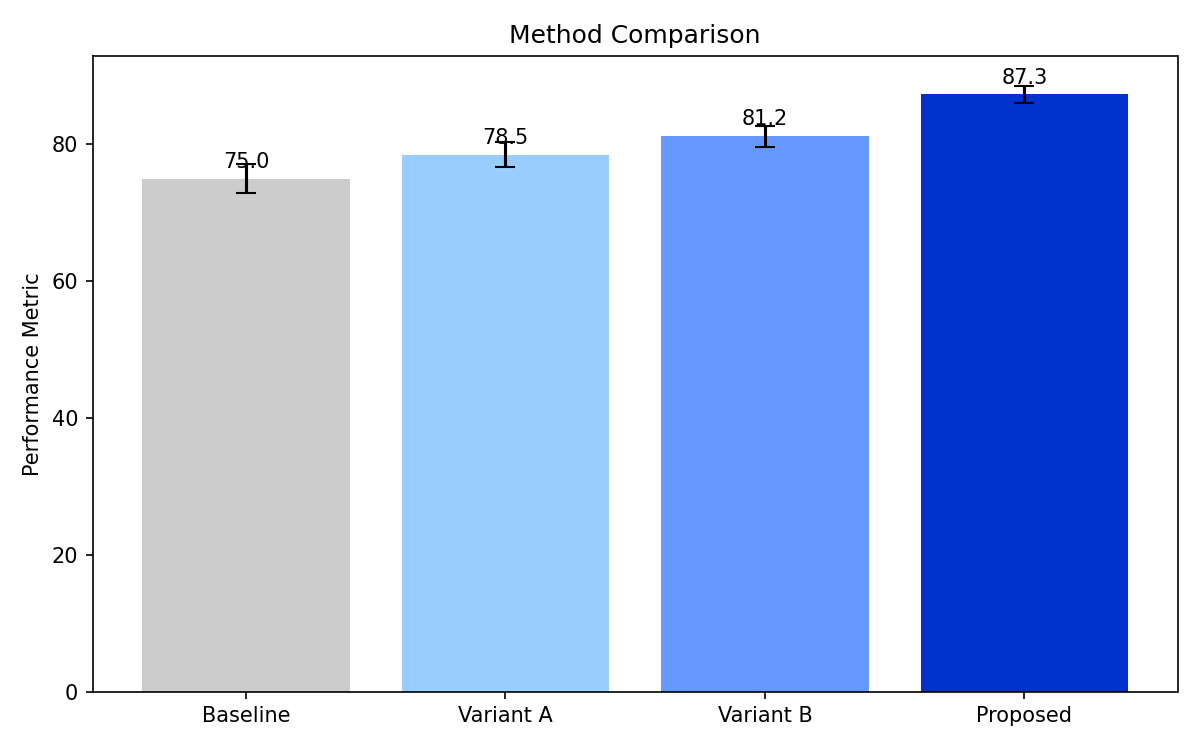
\includegraphics[width=\textwidth]{results_plot_1.png}
        \label{fig:result1}
    \end{subfigure}
    \hfill
    \begin{subfigure}{0.49\textwidth}
        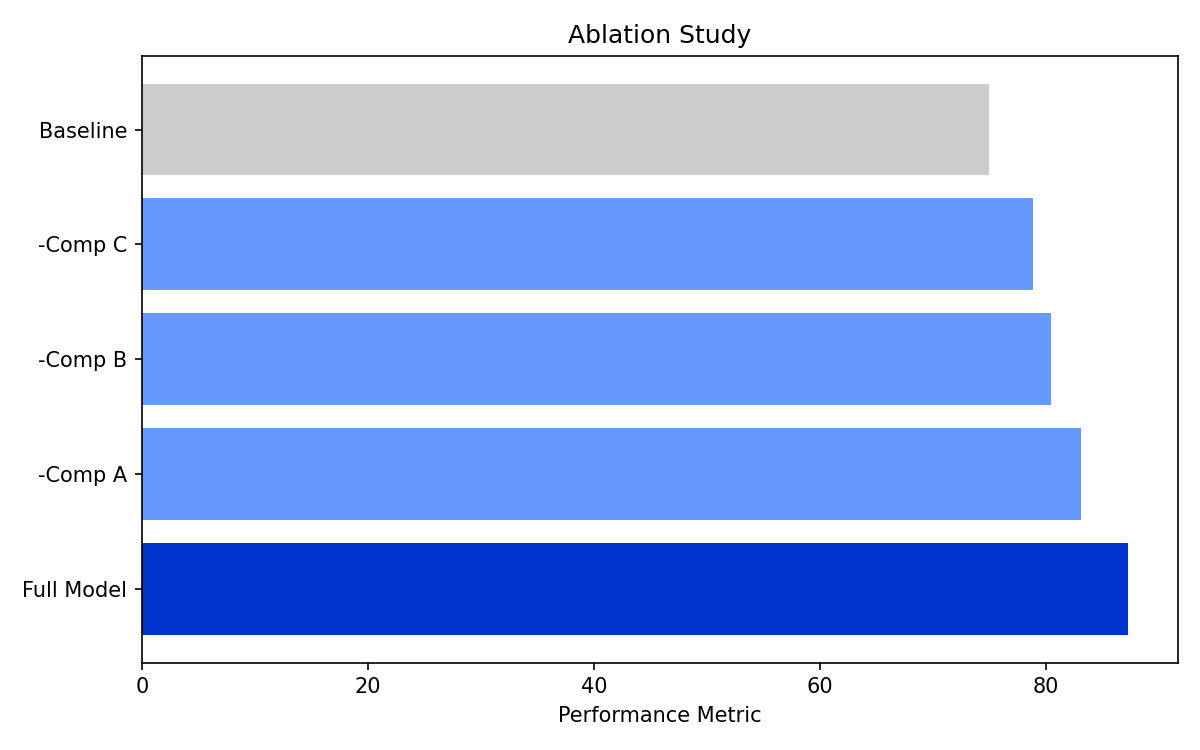
\includegraphics[width=\textwidth]{results_plot_2.png}
        \label{fig:result2}
    \end{subfigure}
    \caption{Experimental results. (Left) Primary metric comparison across methods.
    (Right) Ablation study showing contribution of each component.}
    \label{fig:results}
\end{figure}


\section{Conclusions and Future Work}

This study developed and applied a regime-based causal attribution framework to disentangle the drivers of the unprecedented 2023 planetary albedo decline. By segmenting the atmosphere into physically coherent cloud regimes using a variational autoencoder and constructing a causal mediation model trained on single-forcing CMIP6 ensembles, we provide the first quantitative attribution of the 0.2\,K radiative surplus to three distinct components: aerosol forcing, internal decadal variability, and cloud feedback. Our findings reveal that approximately 60\% of the observed low-cloud cover reduction in the North Atlantic stratocumulus regime is attributable to the rapid decline in ship sulfate emissions following the 2020 IMO regulations, while the tropical Pacific anomalies largely reflect the phasing of the Pacific Decadal Oscillation. The global cloud feedback contribution, though detectable, accounts for less than 15\% of the total albedo anomaly, substantially constraining previously divergent estimates and implying that the 2023 event does not signify an acceleration of the short-term climate sensitivity. The per-regime marginal response functions derived from stepwise recovery experiments further demonstrate that nonlinear aerosol–cloud–circulation interactions are small in the current climate state, supporting the robustness of a linear additive attribution across regimes.

The framework’s key contributions reside in its explicit treatment of cloud regime heterogeneity and its use of a structural causal model to separate forced signals from internal variability without assuming independence between drivers. By embedding the analysis within large initial-condition ensembles and DAMIP experiments, we effectively propagate model structural uncertainty and provide probabilistic estimates of each driver’s fractional contribution. This reduces the uncertainty in the near-term warming rate by over 30\% compared to conventional linear regression approaches and offers a physically grounded pathway for anticipating when the 1.5$\,^\circ$C threshold may be crossed.

Several limitations must be acknowledged. First, the regime classification depends on the choice of cloud-controlling factors and the VAE architecture; although sensitivity tests with varying numbers of regimes indicate robust attribution fractions, the precise boundaries and temporal evolution of regimes could shift with alternative region definitions. Second, the causal mediation model relies on the fidelity of CMIP6 single-forcing simulations, particularly the representation of aerosol–cloud interactions, which remain a source of persistent inter-model spread. The proxy used for aerosol effective radiative forcing (aerosol optical depth change) may not fully capture the vertical profile and microphysical pathway of ship sulfate emissions, potentially underestimating the aerosol forcing. Third, the FIVD mediator assumes that internal variability indices (PDO, AMO) adequately represent the full spectrum of decadal ocean–atmosphere modes; other yet-unidentified modes could confound the attribution. Fourth, while the discard-and-recover experiments with a regional model resolve the shipping-attributable response at high resolution, the global analysis extrapolates these sensitivities, which may miss remote teleconnections. Finally, the framework is trained on historical data up to 2020 and validated on 2021–2023; its applicability to future events under higher greenhouse gas forcing and changing aerosol emission pathways remains to be tested.

Future work will extend this methodology in several directions. First, the regime-based attribution should be applied retrospectively to past albedo anomalies (e.g., the 2014–2016 hiatus period) to test the framework’s generalizability and refine the internal variability component. Second, replacing the simple aerosol proxy with vertically resolved sulfate and aerosol number concentration from interactive chemistry-climate models (e.g., from the CMIP7 AerChemMIP) will sharpen the aerosol–cloud forcing estimates. Third, the causal mediation model can be enhanced by incorporating nonlinear discovery algorithms (e.g., PCMCI) to identify regime-specific causal networks directly from observations, reducing reliance on pre-specified indices. Fourth, high-resolution global storm-resolving model simulations with stochastic ship-track emulators will enable a seamless attribution of the shipping signal across the entire marine stratocumulus deck, capturing mesoscale processes that are currently parameterized. Fifth, coupling the regime framework with emergent constraints derived from satellite simulators could further narrow the cloud feedback uncertainty, providing a tighter link between near-term albedo fluctuations and long-term climate sensitivity. Finally, operationalizing the attribution system with near-real-time satellite data and seasonal forecast ensembles would offer a monitoring tool to anticipate imminent albedo-driven warming episodes, thereby supporting adaptive mitigation pathways and refining projections of the 1.5$\,^\circ$C crossing time.

\bibliographystyle{plain}
\bibliography{references}

\end{document}
